\documentclass[12pt]{exam}
\usepackage{amsthm}
\usepackage{libertine}
\usepackage[utf8]{inputenc}
\usepackage[margin=1in]{geometry}
\usepackage{amsmath,amssymb}
\usepackage{multicol}
\usepackage[shortlabels]{enumitem}
\usepackage{siunitx}
\usepackage{cancel}
\usepackage{graphicx}
\usepackage{pgfplots}
\usepackage{listings}
\usepackage{tikz}
\usepackage{graphicx}
\graphicspath{ {images/} }


\pgfplotsset{width=10cm,compat=1.9}
\usepgfplotslibrary{external}
\tikzexternalize

\newcommand{\class}{Lenguajes de Programaci\'on} % This is the name of the course 
\newcommand{\examnum}{Tarea 02} % This is the name of the assignment
\newcommand{\examdate}{7 de septiembre del 2022} % This is the due date
\newcommand{\timelimit}{}





\begin{document}
\pagestyle{plain}
\thispagestyle{empty}

\noindent
\begin{tabular*}{\textwidth}{l @{\extracolsep{\fill}} r @{\extracolsep{6pt}} l}
\textbf{\class} & \textit{Juan Carlos Faz Leal}\\ %Your name here instead, obviously 
\textbf{\examnum} &&\\
\textbf{\examdate} &&\\
\end{tabular*}\\
\rule[2ex]{\textwidth}{2pt}
\usepackage[document]{ragged2e}
% ---




\begin{enumerate} %You can make lists!

\item Problema 5: La llamada (bundle ’(”a” ”b” ”c”) 0) es un buen uso de bundle? ¿qu\'e produce? ¿por qu\'e?

\begin{verbatim}
(define (bundle s n)
  (cond
    [(null? s) null]
    [else (cons (implode (take s n)) (bundle (drop s n) n))]))
    
\end{verbatim}
\\
\\
\justifying
si decimos que ’(”a” ”b” ”c”) es nuestra lista
de cadanas unitarias, y n es el numero de trozos.
Entonces no tiene sentido que partamos en 0
trozos, por lo que nuestra llamada recursiva
entraria en un ciclo infinito.

\item Problema 9: Dibuja un diagrama como el de la figura anterior pero para la lista '(11 9 2 18 12 14 4 1).

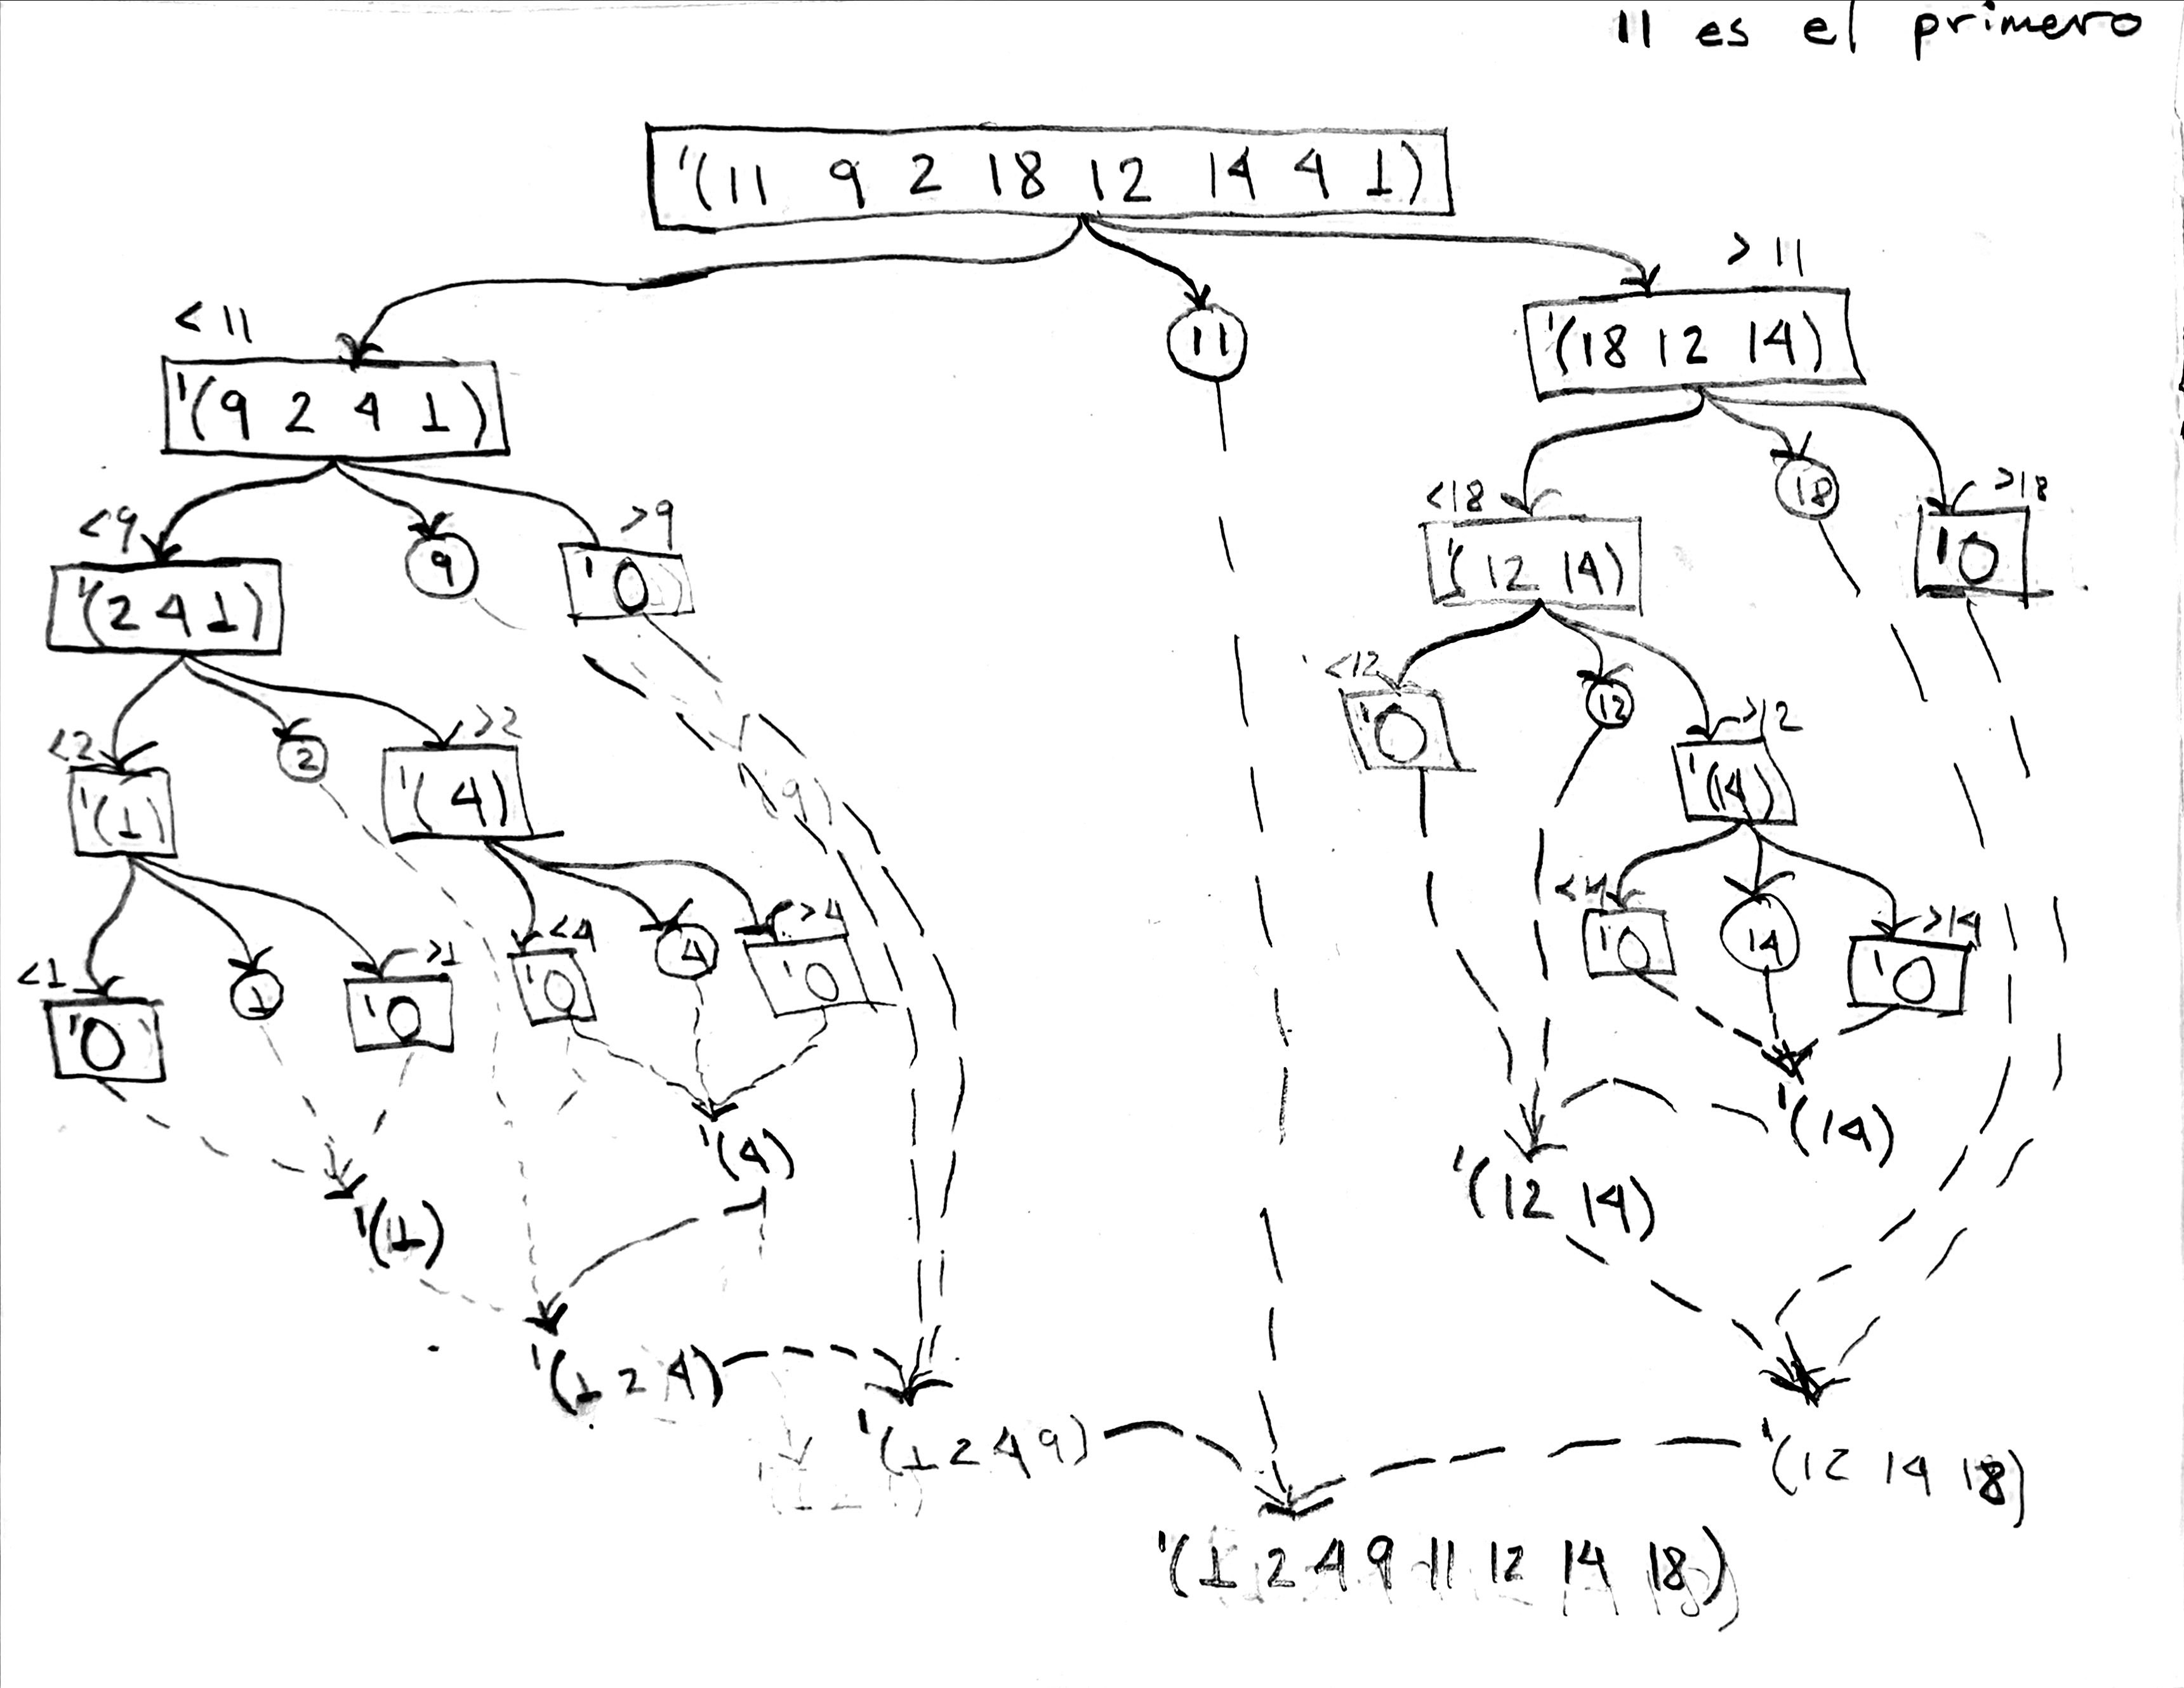
\includegraphics[width=16cm, height=10cm]{Problema 9.jpeg}

\item Problema 11: Si la entrada a quicksort contiene varias repeticiones de un número, va a regresar una lista estrictamente más corta que la entrada. Responde el por qué y arregla el problema.

\justifying
Si usamos el mismo procedimiento que en el problema 9, vemos que se cumple lo que dice el problema.

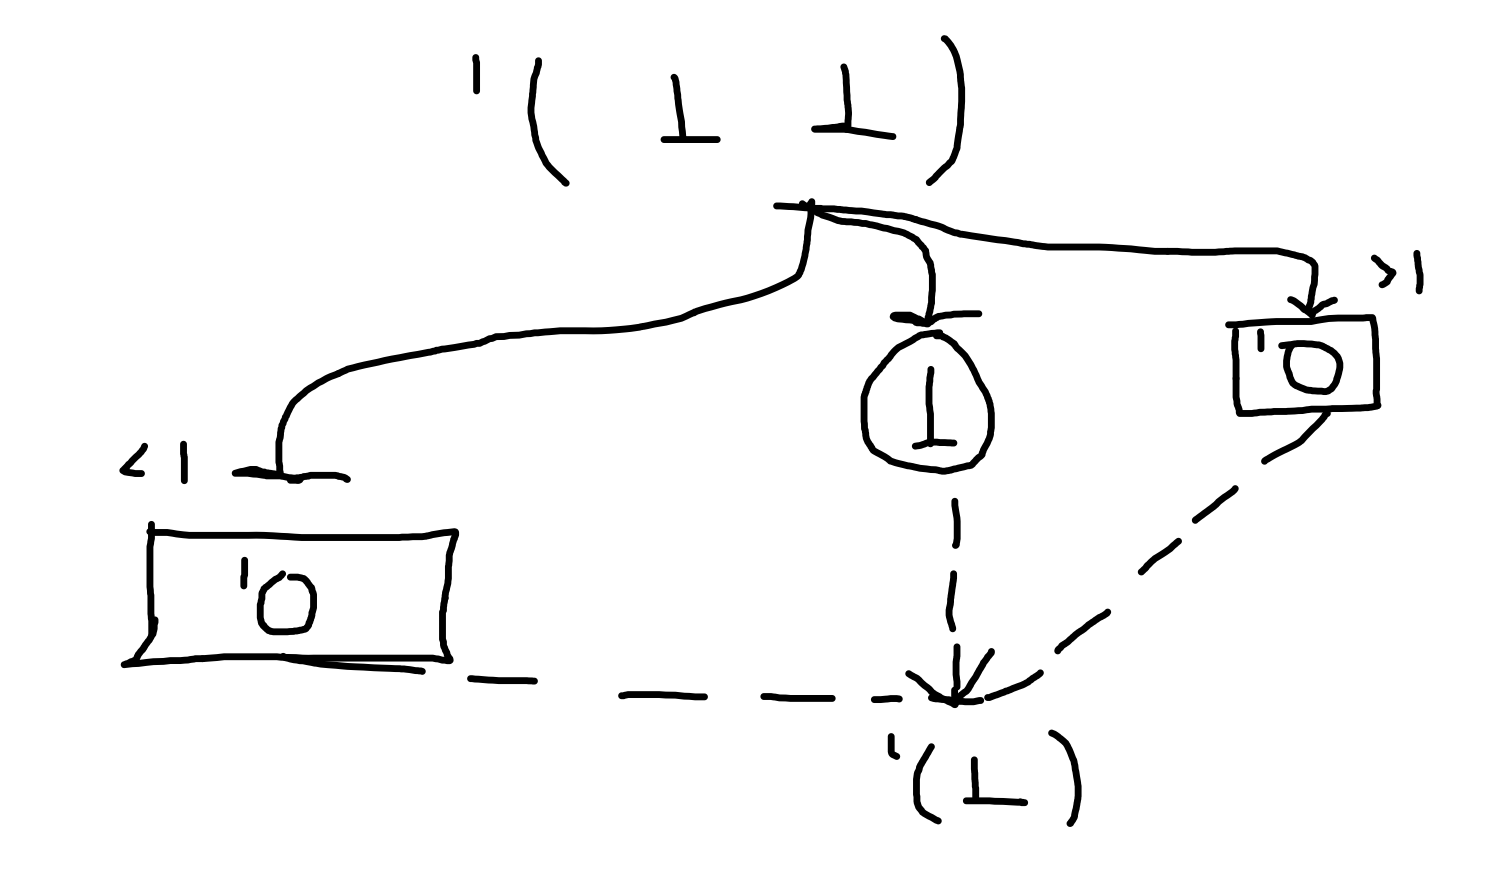
\includegraphics[width=10cm, height=6cm]{Problema 11.png}

\justifying
Al final la lista queda mas chica que la original. Esto pasa porque el metodo se compone de 3 cosas:

\begin{enumerate}
    \item Los menores al pivote.
    \item El pivote.
    \item Los mayores al pivote
\end{enumerate}

\justifying
Cuando nosotros tomamos al primer elemento (que en este caso es: 1) como nuestro pivote, debemos hacer las comparaciones mencionadas anteriormente (los menores y los mayores). Entonces tomamos el segundo elemento y lo comparamos, como el 1 no es mayor, ni menor que el 1, si no que es igual. Por tanto tenemos que es un '0 en los mayores y '0 en los menores. Por lo que al final solo queda el pivote.
\\
\\
\justifying
Para solucionar el problema prodriamos verificar si el pivote se repite en la lista, y si es asi, entonces tomar con el elemento pivote, como una lista donde aparece el pivote tantas veces como se repite.

\end{enumerate}

\end{document}
